\subsection{27 августа. Пер. Перемётный (1А)}
\textit{Метеоусловия: утром, днём, вечером ясно, тепло.}

\begin{figure}[h!]
	\centering
	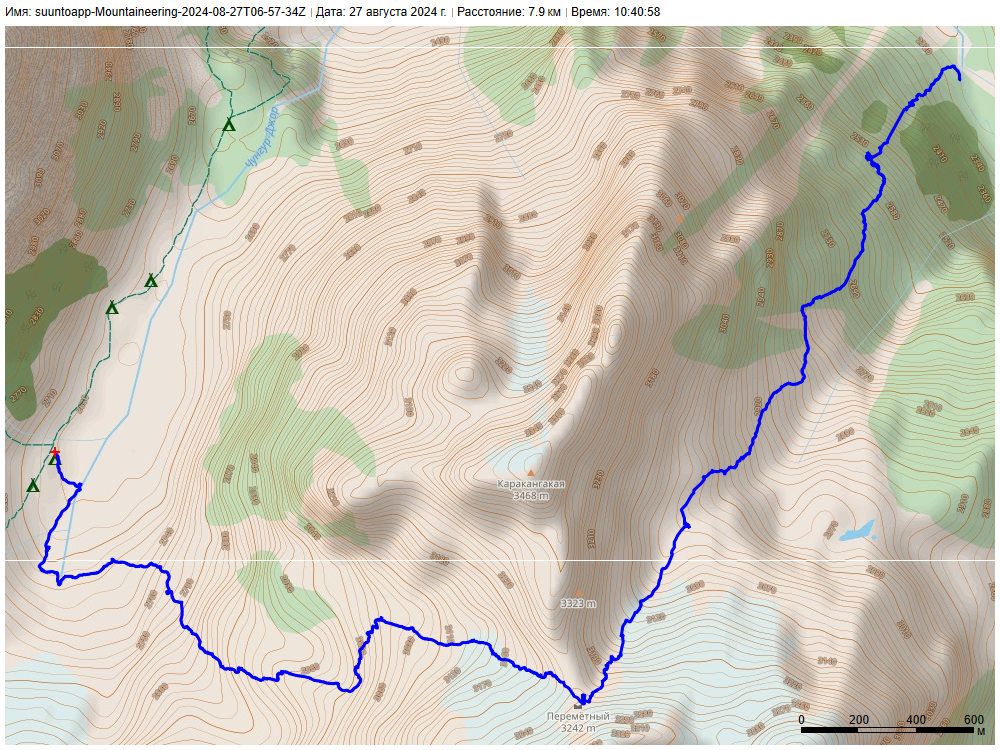
\includegraphics[angle=0, width=0.7\linewidth]{../pics/mini_maps/27}
	\label{fig:mini_27}
\end{figure}




\begin{figure}[h!]
	\centering
	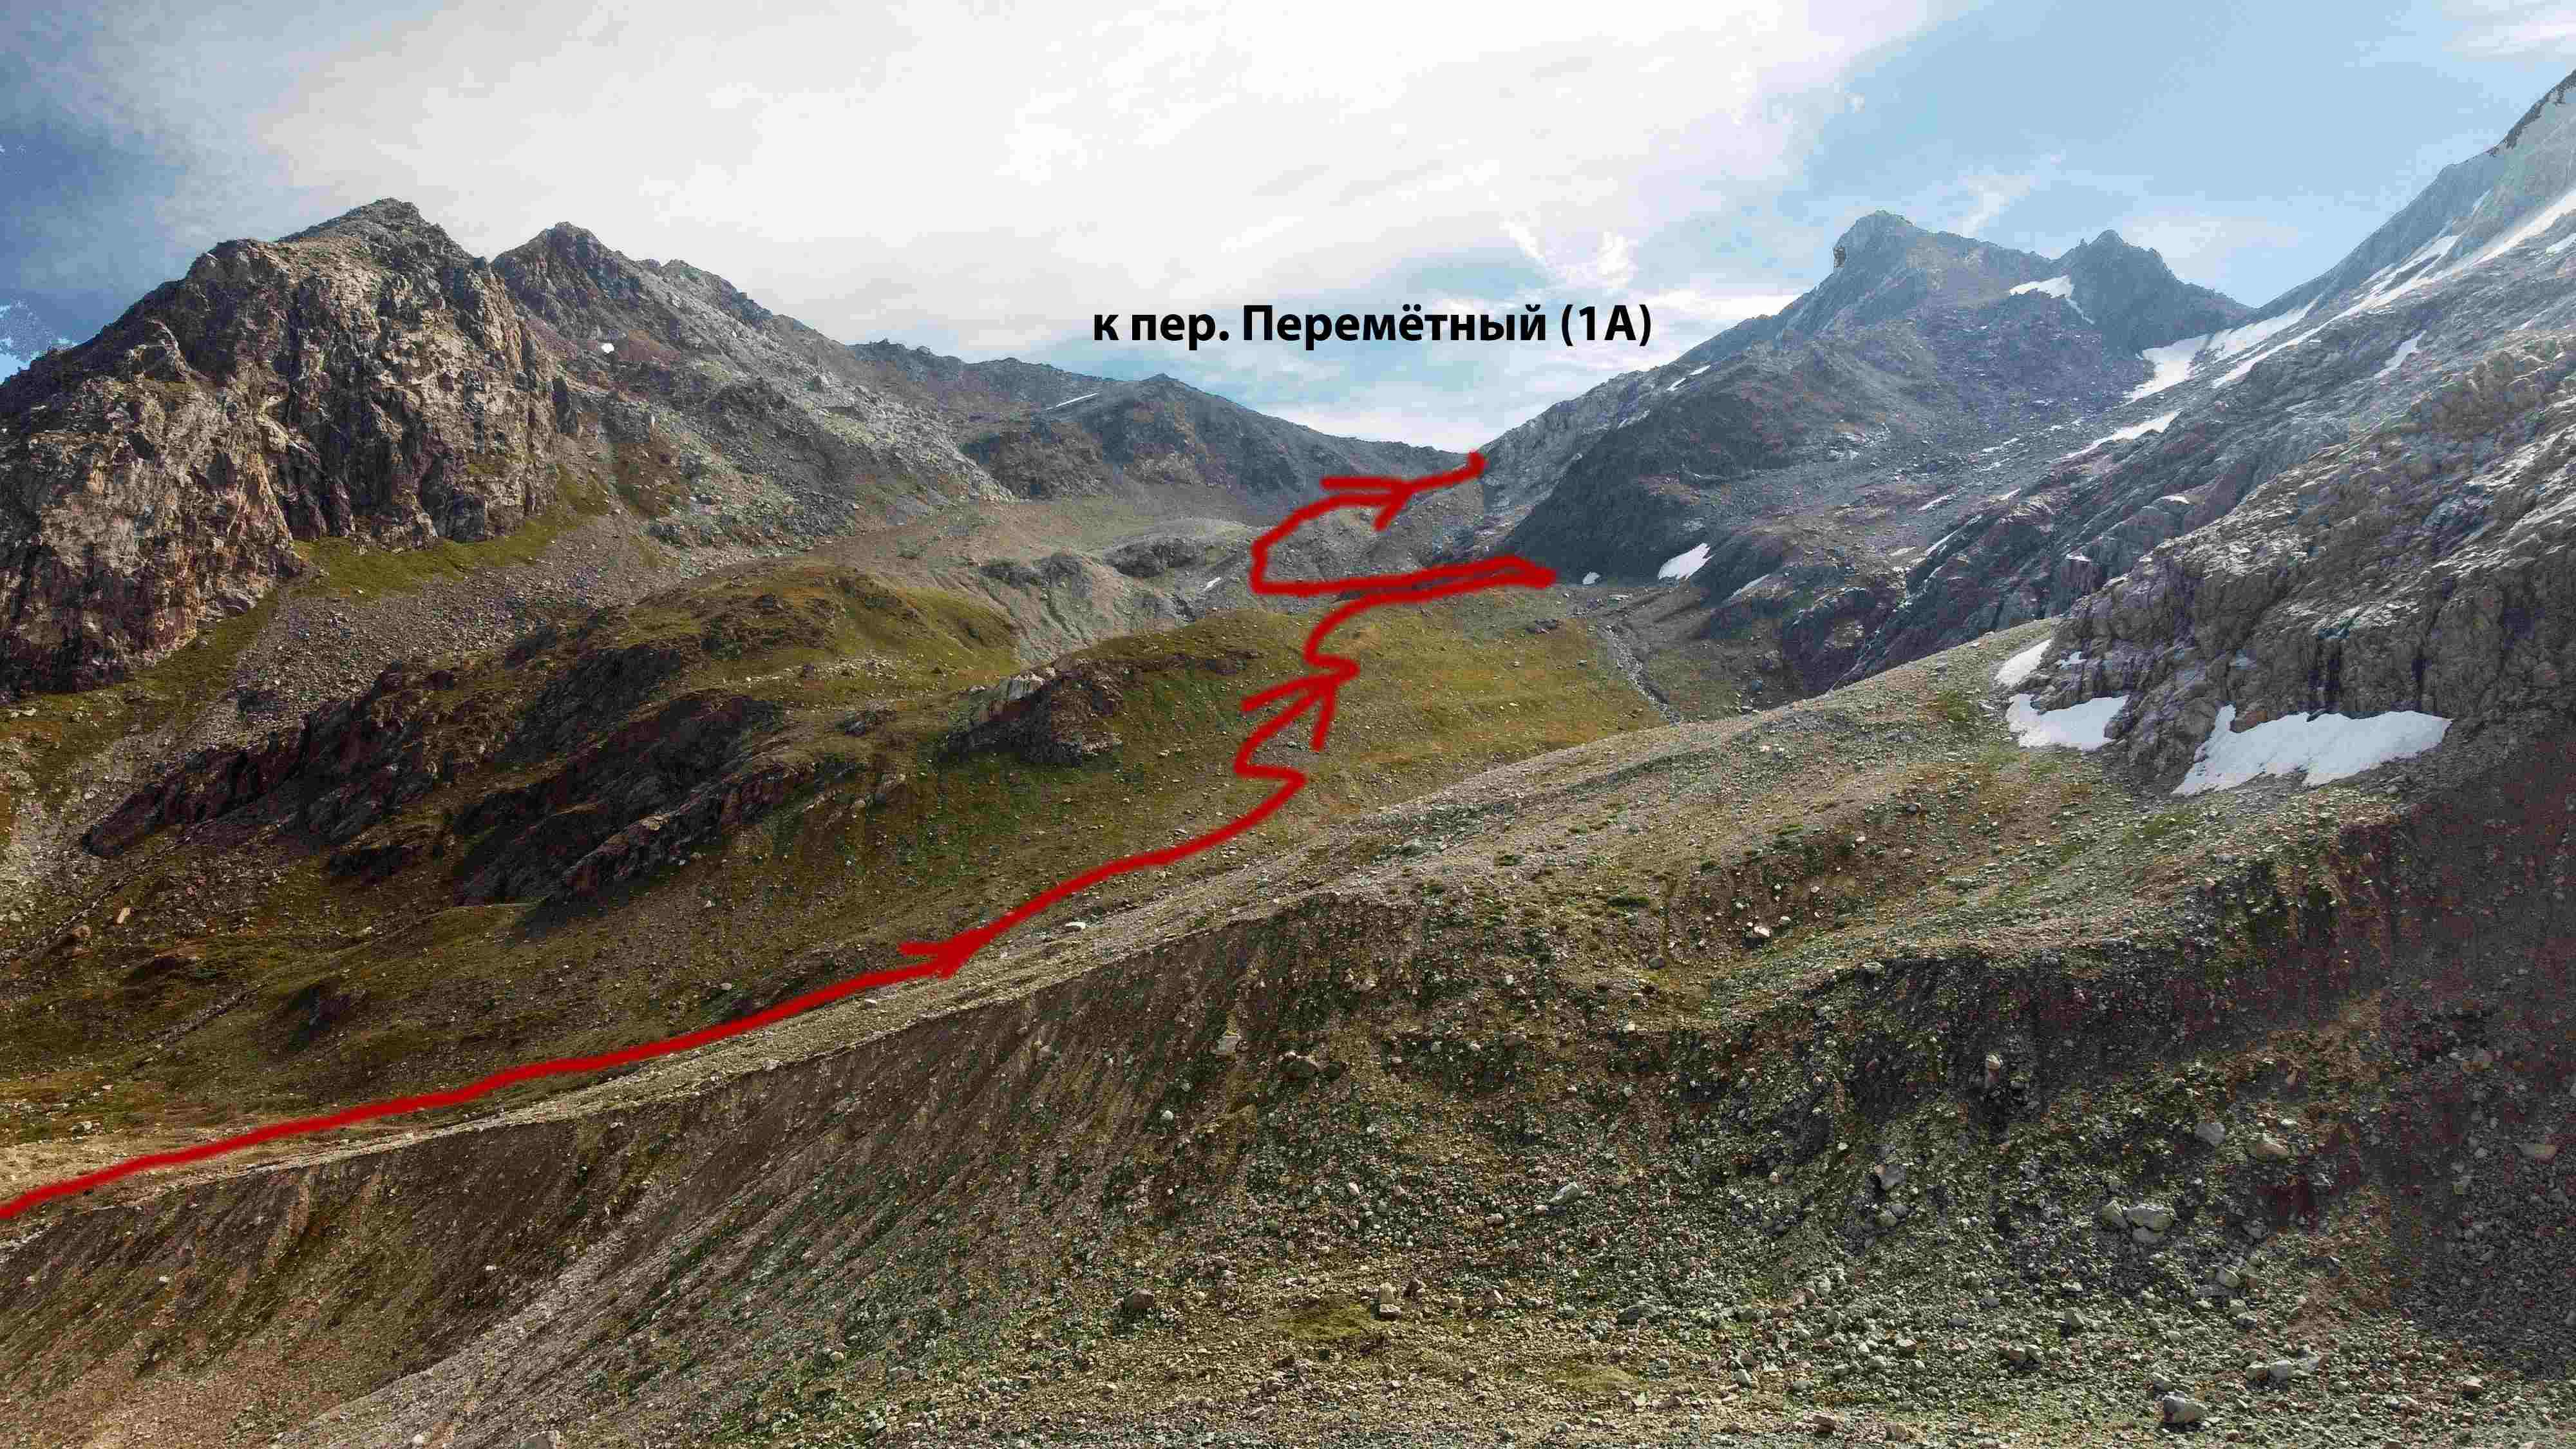
\includegraphics[width=0.7\linewidth]{../pics/perem_1}
	\caption{Начало подъёма к пер. Перемётный из д.р. Чунгур-Джар}
	\label{fig:perem_1}
\end{figure} 


Метеоусловия: солнечно, тепло

Утром долго стирались, чинились и сушились, руковод курил какао и размышлял... Переметный было решено брать!

*картинка с утренним лагерем*

Задача номер раз: перейти многорукаавье реки Чунгур-Джар. Оказалось сложнее, чем казалось. Часть группы промочила ботинки и усердно их сушила на каждом привале.

*картинка с руслом*

Задача номер два: пройти подъем на перевал. Поднялись на морену, прошли по гребню. На высоте 2410м (N 43.24135\degree, E 42.24827\degree) начали траверс по сыпухе и под небольшой скалой на соседнюю морену. После этого - прямым курсом на перевал. С задачей два справились в ..
На перевале сняли записку группы туристов из Ростова-на-Дону и Новочеркасска от 20.08.2019. Примечательно, что эта группа в свое время сняла записку Горной секции МФТИ под руководством Королева Андрея от 2018 года - в этот поход ходила руковод.

*картинка с мореной, картинка с перевала*

Задача три: спуститься в низ, в д.р. Чиринкол. Здесь начинается очень интересная и поучительная история.

Вниз сначала шли по сыпухе (нормально), усердно считали моренные валы чтобы не ошибиться и не угодить в березняк. По пути старались расставлять турики, но время подгоняло, в маршруте мы были не  уверены и на полпути мы это дело забросили.  Потом начался травянистый склон, альпеншток альпеншточил на все 100. На высоте ?? м выбрались на курумник, на котором не обошлось без легкого кровопролития. К сумерка снова вышли на травянистый склон. Русло пересохшего ручья, засыпанного крупными камнями, предоставило удобный вариант до спуска. К моменту, когда мы добрались до зарослей рододендронов, уже порядком стемнело, дальше шли с фонарикам. 

В .. вышли на отличную стоянку на берегу реки Чиринкол (N 43.26002, E 42.27489). В .. поужинали, в .. легли спать. С задачей три справились!



\clearpage